\documentclass[12pt]{article}
\usepackage{amsmath, amssymb}
\usepackage{tikz}
\usepackage{geometry}
\geometry{a4paper, margin=1in}
\usepackage{hyperref}
\usepackage{listings}
\usepackage{xcolor}

\lstset{
    language=C++,
    basicstyle=\ttfamily\small,
    keywordstyle=\color{blue},
    commentstyle=\color{green!60!black},
    stringstyle=\color{red}
}

\title{The Ultimate Advanced Geometry Reference for Competitive Programming}
\date{}

\begin{document}
\maketitle
\tableofcontents
\newpage

\section{Points, Lines, Polygons \& Sweep-Line}

\subsection{Convex Hull (Monotone Chain)}
\begin{itemize}
    \item \textbf{Rule:} Sort points lexicographically (first by $x$, then by $y$). Build the lower and upper hulls in two passes using a stack.
    \item \textbf{Formula:} For points $P_1, P_2, P_3$, the 2D cross product is $CP = (P_2.x - P_1.x)(P_3.y - P_1.y) - (P_2.y - P_1.y)(P_3.x - P_1.x)$. Pop $P_2$ from the stack while $CP \le 0$.
\end{itemize}

\begin{center}
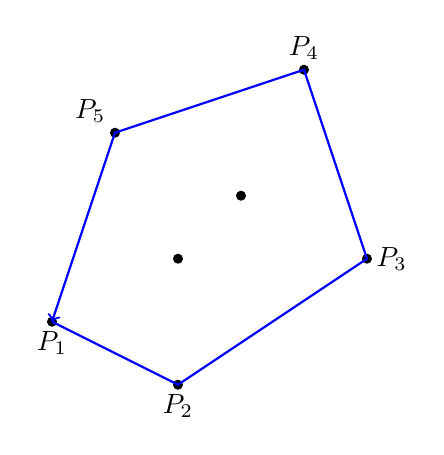
\begin{tikzpicture}[scale=0.8]
    \filldraw (0,0) circle (2pt) node[below] {$P_1$};
    \filldraw (2,-1) circle (2pt) node[below] {$P_2$};
    \filldraw (5,1) circle (2pt) node[right] {$P_3$};
    \filldraw (4,4) circle (2pt) node[above] {$P_4$};
    \filldraw (1,3) circle (2pt) node[above left] {$P_5$};
    \filldraw (2,1) circle (2pt); % interior
    \filldraw (3,2) circle (2pt); % interior
    \draw[thick, blue, ->] (0,0) -- (2,-1) -- (5,1) -- (4,4) -- (1,3) -- (0,0);
\end{tikzpicture}
\end{center}

\subsection{Point-in-Polygon (Ray Casting)}
\begin{itemize}
    \item \textbf{Ray Casting Rule:} Cast a horizontal ray from the point to $+x$. Count edge intersections. Odd = inside, Even = outside.
    \item \textbf{Edge-Cases:} Only count an intersection if the edge crosses the ray strictly (e.g., $y_{\min} \le P.y < y_{\max}$) to avoid double counting at vertices.
\end{itemize}

\subsection{Half-Plane Intersection (Polygon Kernel)}
\begin{itemize}
    \item \textbf{Representation}: $ax + by + c \le 0$, defined as a directed line where the valid region is strictly to its "left".
    \item \textbf{Bounding Box Trick}: Add 4 lines forming a massive bounding box (e.g., $[-INF, INF]$) to force a bounded region.
    \item \textbf{Algorithm $\mathcal{O}(N \log N)$}: Sort lines by polar angle \texttt{atan2(dy, dx)}. Maintain a \texttt{deque} of lines. For a new line, \texttt{pop\_back} while the intersection point of the last two lines is strictly outside (to the right of) the new line. Do the same for \texttt{pop\_front}. Finally, verify the deque forms a valid polygon.
\end{itemize}

\subsection{Voronoi Diagrams \& Delaunay Triangulation (DT)}
\begin{itemize}
    \item \textbf{Empty Circumcircle Property}: A triangulation is Delaunay iff the circumcircle of every triangle contains no other input points in its interior.
    \item \textbf{Nearest Neighbors}: The nearest neighbor graph is a strict subgraph of the DT.
    \item \textbf{InCircle Test (Robust Predicates)}: To check if a point $D$ is inside the circumcircle of counter-clockwise $\triangle ABC$, the determinant of the $4 \times 4$ matrix $[x, y, x^2+y^2, 1]$ for points $A, B, C, D$ must be $> 0$.
\end{itemize}

\subsection{Welzl's Algorithm (Minimum Enclosing Circle)}
\begin{itemize}
    \item \textbf{Expected $\mathcal{O}(N)$ Trick}: You \textbf{must} randomly shuffle the input points before running the algorithm.
    \item \textbf{Math}: The MEC is uniquely determined by either 2 points (forming the diameter) or 3 points (forming the circumcircle). For $A, B, C$, let $a = B-A$, $b = C-A$. Center $= A + \frac{(\|a\|^2 b - \|b\|^2 a)^\perp}{2 (a_x b_y - a_y b_x)}$.
\end{itemize}

\subsection{Point Location in Planar Subdivisions}
\begin{itemize}
    \item \textbf{Offline Queries (Sweep-Line $\mathcal{O}((N+Q)\log N)$)}: Sort points by X-coordinate. Maintain active non-intersecting edges in a Y-ordered \texttt{std::set}. Query by \texttt{upper\_bound} to find bounding edges.
    \item \textbf{Fractional Cascading Basics}: Used to optimize multiple binary searches from $\mathcal{O}(\log^2 N)$ to $\mathcal{O}(\log N)$ by storing pointers between adjacent slab data structures.
\end{itemize}

\subsection{Shoelace and Pick's Theorem}
\begin{itemize}
    \item \textbf{Shoelace Formula:} Area = $\frac{1}{2} \left| \sum_{i=1}^{n} (x_i y_{i+1} - x_{i+1} y_i) \right|$. Gives signed area.
    \item \textbf{Pick's Theorem:} Area = $I + \frac{B}{2} - 1$.
\end{itemize}

\section{Circles and Triangles}

\subsection{Circle-Circle Intersection}
\begin{itemize}
    \item \textbf{Condition:} Let $d = \|P_1 - P_0\|$. Intersect if $|r_0 - r_1| \le d \le r_0 + r_1$.
    \item \textbf{Vector Approach:} Radical axis distance $a = \frac{r_0^2 - r_1^2 + d^2}{2d}$. Altitude $h = \sqrt{r_0^2 - a^2}$.
\end{itemize}

\begin{center}
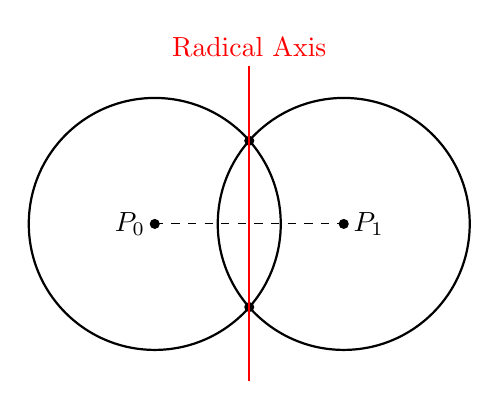
\begin{tikzpicture}[scale=0.8]
    \draw[thick] (0,0) circle (2cm);
    \draw[thick] (3,0) circle (2cm);
    \filldraw (0,0) circle (2pt) node[left] {$P_0$};
    \filldraw (3,0) circle (2pt) node[right] {$P_1$};
    \draw[dashed] (0,0) -- (3,0);
    \filldraw (1.5,1.32) circle (2pt);
    \filldraw (1.5,-1.32) circle (2pt);
    \draw[red, thick] (1.5, -2.5) -- (1.5, 2.5) node[above] {Radical Axis};
\end{tikzpicture}
\end{center}

\subsection{Triangle Centers \& Fermat Point}
\begin{itemize}
    \item \textbf{Incenter ($I$):} Intersection of angle bisectors. $I = (\frac{ax_1 + bx_2 + cx_3}{a+b+c}, \frac{ay_1 + by_2 + cy_3}{a+b+c})$.
    \item \textbf{Orthocenter ($H$):} Use the Euler Line property. $H = 3G - 2O$.
    \item \textbf{Fermat Point}: Minimizes $PA + PB + PC$. If any angle $\ge 120^\circ$, it is that vertex. Otherwise, $\angle APB = \angle BPC = \angle CPA = 120^\circ$. \textbf{Trick:} The distance sum is strictly convex; use Ternary Search or Simulated Annealing.
\end{itemize}

\subsection{Nine-Point Circle \& Simson Line}
\begin{itemize}
    \item \textbf{Nine-Point Circle}: Passes through 9 distinct points (midpoints of sides, altitude feet, midpoints from $H$ to vertices). Center $N$ is the exact midpoint of $HO$. Radius is $R/2$.
    \item \textbf{Simson Line}: The feet of perpendiculars from a point $P$ to the sides of $\triangle ABC$ are collinear \textbf{iff} $P$ lies on the circumcircle. The Simson line for $P$ strictly bisects the segment $PH$ on the Nine-Point Circle.
\end{itemize}

\subsection{The Apollonius Problem}
\begin{itemize}
    \item \textbf{Goal}: Find a circle tangent to three given circles. (Algebraically creates 8 sign combinations).
    \item \textbf{CP Trick (Circle Inversion)}: Shrink the smallest circle to a point by subtracting its radius from the others. Perform geometric inversion centered at this point. Find common tangents to the two new circles/lines, and invert the tangents back!
\end{itemize}

\section{Spherical Geometry}
\begin{itemize}
    \item \textbf{Haversine Formula}: For shortest distance on a sphere surface to avoid catastrophic precision loss:
    $$a = \sin^2\left(\frac{\Delta\varphi}{2}\right) + \cos\varphi_1 \cos\varphi_2 \sin^2\left(\frac{\Delta\lambda}{2}\right)$$
    $$d = 2R \cdot \text{atan2}(\sqrt{a}, \sqrt{1-a})$$
    \item \textbf{CP Trick}: Always use \texttt{atan2(y, x)} across all distances. It prevents \texttt{NaN} errors compared to raw \texttt{acos}.
\end{itemize}

\section{3D Geometry \& Transformations}

\subsection{3D Vector Math}
\begin{itemize}
    \item \textbf{Dot Product:} $V_1 \cdot V_2 = x_1x_2 + y_1y_2 + z_1z_2$. ($0$ = orthogonal).
    \item \textbf{Cross Product:} $V_1 \times V_2 = (y_1z_2 - z_1y_2, \ z_1x_2 - x_1z_2, \ x_1y_2 - y_1x_2)$. Magnitude equals parallelogram area.
    \item \textbf{Triple Scalar Product:} $V_1 \cdot (V_2 \times V_3)$. Gives signed volume of the parallelepiped. ($0$ = coplanar).
\end{itemize}

\subsection{Distance Between 3D Skew Lines}
\begin{itemize}
    \item \textbf{Lines}: $L_1 = P_1 + t_1 \vec{D}_1$ and $L_2 = P_2 + t_2 \vec{D}_2$. Common normal $\vec{N} = \vec{D}_1 \times \vec{D}_2$.
    \item \textbf{Distance Formula}: $d = \frac{|(P_2 - P_1) \cdot (\vec{D}_1 \times \vec{D}_2)|}{|\vec{D}_1 \times \vec{D}_2|}$.
\end{itemize}

\subsection{3D Polyhedron Volume}
\begin{itemize}
    \item \textbf{Tetrahedron}: $V = \frac{1}{6} |(B-A) \cdot ((C-A) \times (D-A))|$.
    \item \textbf{Polyhedron (3D Shoelace)}: Triangulate faces with consistent CCW order (outward-facing normals). For each face $A,B,C$, compute $V_{face} = \frac{1}{6} (A \cdot (B \times C))$. Total Volume = $|\sum V_{face}|$.
\end{itemize}

\subsection{Affine Transformation Matrices (Homogeneous Coordinates)}
\begin{itemize}
    \item \textbf{Representation}: Points are $[x,y,z,1]^T$, vectors are $[x,y,z,0]^T$. 
    \item \textbf{Translation}: Diagonal $1$s, $4$th column is $(t_x, t_y, t_z, 1)$.
    \item \textbf{Rotation \& Scaling}: Adjust the top-left $3 \times 3$ matrix.
    \item \textbf{Trick}: Combine multiple transformations by multiplying their matrices in \textbf{reverse order} of application ($M = T \times R$). Apply via $M \times P$.
\end{itemize}

\end{document}
